\pagebreak
\section{Manufactured Solutions}
Discretize the one-dimensional advection-diffusion equation, $u_t + au_x - \nu u_{xx}= 0$, using the trapezoidal method in time and second-order central differences in space. Assume a grid of length $L$, periodic boundaries, and $N$ spatial intervals.


\begin{enumerate}[label=\alph*., start = 1]
    \item Write a computer program that implements the given method, and run a simulation using the parameters given in problem 2c, $\nu= 0.1,\ N= 64$, and a CFL number of $\sigma= 0.5$.  Plot the state at the final time, $u(x,T)$.
    
    \begin{align*}
        \shortintertext{First starting with the expressions for the expansions one-dimensional advection-diffusion equation gives,}
        u_{j}^{n+1} & = u_j^n + \frac{\Delta t}{2}\left(f^{n+1} + f^n\right)\\
        u_x & = \frac{u_{j+1}^n - u_{j-1}^n}{2\Delta x}\\
        u_{xx} & = \frac{u_{j-1}^n - 2u_{j}^n + u_{j+1}^n}{\Delta x^2}\\
        \shortintertext{Substituting in and solve for $u_t$ gives,}
        u_t & = \nu \frac{u_{j-1}^n - 2u_{j}^n + u_{j+1}^n}{\Delta x^2} - a\frac{u_{j+1}^n - u_{j-1}^n}{2\Delta x} = \dot{u} = f = \doubleunderline{A}u_j^n\\
        \doubleunderline{A}u_j^n & = -\frac{2\nu}{\Delta x^2}u_j^n + \left(\frac{\nu}{\Delta x^2} + \frac{a}{2\Delta x}\right)u_{j-1}^n + \left(\frac{\nu}{\Delta x^2} - \frac{a}{2\Delta x}\right)u_{j+1}^n\\
        \shortintertext{Using this relationship of $\doubleunderline{A}$, solve for the update relationship for $u^{n+1}_j$,}
        u_j^{n+1} - \frac{\Delta t}{2}f^{n+1} & = u_j^{n} + \frac{\Delta t}{2}f^{n} \\
        u_j^{n+1} - \frac{\Delta t}{2}\doubleunderline{A}u^{n+1} & = u_j^{n} + \frac{\Delta t}{2}\doubleunderline{A}u^{n} \\
        \left(\doubleunderline{I} - \frac{\Delta t}{2}\doubleunderline{A}\right)u_j^{n+1} & = \left(\doubleunderline{I} + \frac{\Delta t}{2}\doubleunderline{A}\right)u_j^{n}\\
    \end{align*}

    \vspace{-0.5in}
    \begin{equation*}
        \boxed{u_j^{n+1}  = \left(\doubleunderline{I} - \frac{\Delta t}{2}\doubleunderline{A}\right)^{-1}\left(\doubleunderline{I} + \frac{\Delta t}{2}\doubleunderline{A}\right)u_j^n}
    \end{equation*}

    \vfill
    \begin{flushleft}
        Continued on next page \ldots
    \end{flushleft}

    \pagebreak
    Implementing the trapezoidal method derived above and implementing into Matlab with the given parameters above, I generate Figure \ref{fig:q3a} shown below.

    \begin{figure}[h]
        \centering
        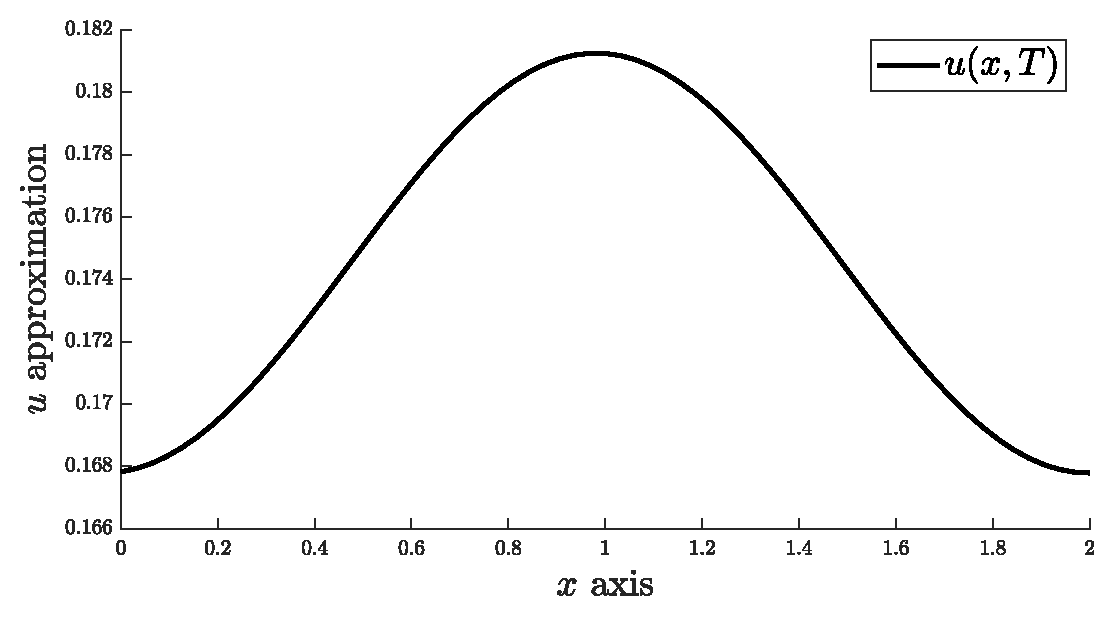
\includegraphics[width = 0.9\linewidth]{q3/q3a.eps}
        \caption{Implementation of trapezoidal method.}
        \label{fig:q3a}
    \end{figure}

    \begin{fminipage}{0.9\linewidth}
        \textbf{Shown above in Figure \ref{fig:q3a}, is the approximated solution through implementation of of the trapezoidal method. This shows the solution after one period which should return the initial condition decayed by some exponential factor.}
    \end{fminipage}
\end{enumerate}

\pagebreak
\begin{enumerate}[label=\alph*., start = 2]
    \item Apply the method of manufactured solutions to your discretization.  The PDE will now need a source term: $u_t+au_x - \nu u_{xx}=s(x,t)$. Derive the form of $s(x,t)$ for the manufactured solution $u^{MS}= \sin{(kx -\omega t)}$, where $k$ and $\omega$ are known constants.
    
    \vspace{-0.35in}
    \begin{align*}
        \shortintertext{Using the manufactured solution, and substituting in the expression for the PDE I get,}
        s(x,t) & = \frac{\partial}{\partial t}u^\text{MS} + a\frac{\partial}{\partial x}u^\text{MS} - \nu \frac{\partial^2}{\partial x^2}u^\text{MS}\\
        s(x,t) & = -\omega\cos{(kx - \omega t)} + ak\cos{(kx-\omega t)} + \nu k^2\sin{(kx-\omega t)}\\
        \shortintertext{Condensing and simplfying the solution for $s(x,t)$ further gives,}
    \end{align*}

    \vspace{-0.5in}
    \begin{equation*}
        \boxed{s(x,t) = \left(ak - \omega\right)\cos{(kx - \omega t)} + \nu k^2\sin{(kx-\omega t)}\\}
    \end{equation*}

    \vspace{-0.45in}
    \begin{align*}
        \shortintertext{Since we are implementing the trapezoidal method, we take the average in time such that,}
        \underline{s} & = \frac{\Delta t}{2}\left(s(x,t^{n+1}) + s(x,t^{n})\right)\\
        \shortintertext{Then following the steps from part a. but with the additional source term gives,}
        u_j^{n+1} & = \left(\doubleunderline{I} - \frac{\Delta t}{2}\doubleunderline{A}\right)^{-1}\left( \left(\doubleunderline{I} + \frac{\Delta t}{2}\doubleunderline{A}\right)u^n_j + \underline{s}\right)\\
        \shortintertext{Therefore, the trapezoidal update for $u^{n+1}_j$ is,}
    \end{align*}

    \vspace{-0.35in}
    \begin{equation*}
        \boxed{u_j^{n+1} = \left(\doubleunderline{I} - \frac{\Delta t}{2}\doubleunderline{A}\right)^{-1}\left( \left(\doubleunderline{I} + \frac{\Delta t}{2}\doubleunderline{A}\right)u^n_j + \frac{\Delta t}{2}\left(s(x,t^{n+1}) + s(x,t^{n})\right)\right)\\}
    \end{equation*}

\end{enumerate}

\pagebreak
\begin{enumerate}[label=\alph*., start = 3]
    \item Implement the method of manufactured solutions in your discretization, and present the solution at $t=T=L/a$ for $N= 64,\ \sigma= 0.5$. Use $k=4\pi/L$ and $\omega = 5a/L$.
    
    Using the source term $s(x,t)$ derived in part c. above and implementing through Matlab gives that the final value is below in Figure \ref{fig:q3c}

    \begin{figure}[h]
        \centering
        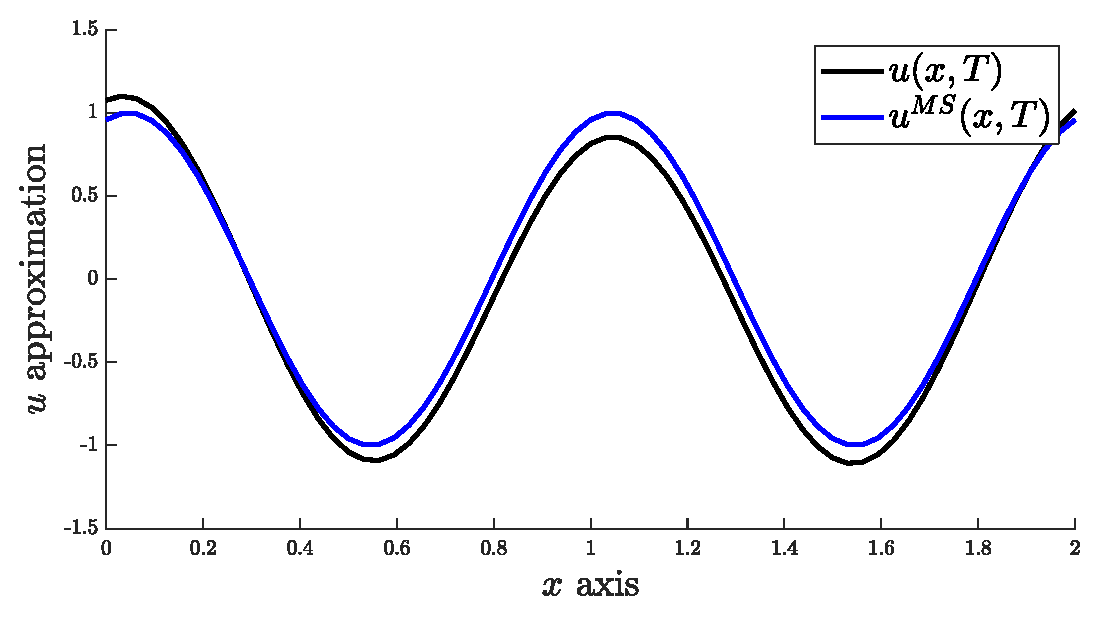
\includegraphics[width = 0.9\linewidth]{q3/q3c.eps}
        \caption{Implementation method of manufactured solutions for $T=L/a, N=64,\ \sigma=0.5$.}
        \label{fig:q3c}
    \end{figure}
    
    \begin{fminipage}{0.9\linewidth}
        \textbf{Looking above to Figure \ref{fig:q3c} and comparing the approximated solution from the trapezoidal method gives that it is close in approximation to the analytical solution (manufactured solution) when $\bf N=64$. At higher values of $\bf N$ the solution is much closer in comparison.}
    \end{fminipage}
    
\end{enumerate}

\pagebreak
\begin{enumerate}[label=\alph*., start = 4]
    \item Using the manufactured solution, perform spatial and temporal convergence studies of your discretization, using the $L_2$ solution error, and verify that the orders of accuracy match your expectations.

    \begin{figure}[h]
        \centering
        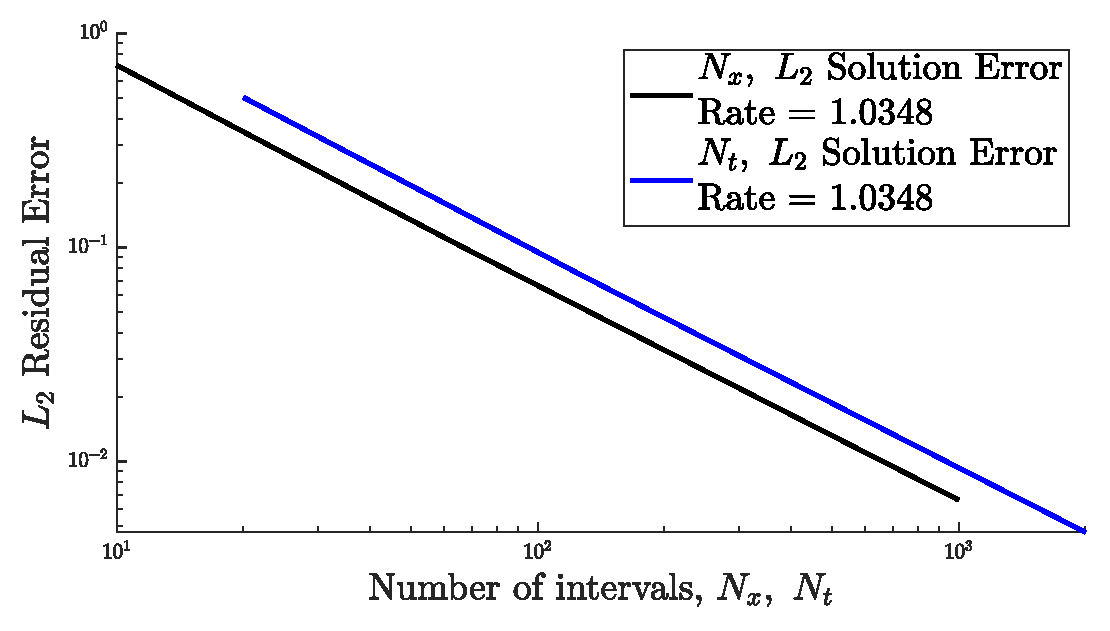
\includegraphics[width = 0.9\linewidth]{q3/q3d.eps}
        \caption{Spatial and temporal convergence study using manufactured solution.}
        \label{fig:q3d}
    \end{figure}

    \begin{fminipage}{0.9\linewidth}
        \textbf{Looking above in Figure \ref{fig:q3d} to the spatial and temporal convergences shows that this is first-order accurate such that $\bf \mathcal{O}(\Delta t)$ when converging.}
    \end{fminipage}

    Tabulating the spatial and temporal solution errors from the graph above gives that the convergences are as follows in Tables \ref{tab:spatial}, \ref{tab:temporal} below confirming first-order accuracy.

    \begin{table}[h]
        \centering
        \begin{minipage}{0.4\linewidth}
            \centering
            \caption{Spatial convergence varying $N_x$}
            \label{tab:spatial}
            \begin{tabular}{l l}
                Rates & Order of accuracy\\\hline
                \input{q3/rates_nx}
            \end{tabular}
        \end{minipage}%
        \begin{minipage}{0.4\linewidth}
            \centering
            \caption{Temporal convergence varying $N_t$}
            \label{tab:temporal}
            \begin{tabular}{l l}
                Rates & Order of accuracy\\\hline
                \input{q3/rates_nt}
            \end{tabular}
        \end{minipage}
    \end{table}


\end{enumerate}